\section{Implementación del sistema ANPR-VISION}
\label{sec:implementacion}

A partir de la metodología descrita en la Sección~\ref{sec:metodologia}, esta sección detalla cómo se materializó la arquitectura propuesta en un prototipo funcional. La implementación de ANPR-VISION se estructura alrededor de cuatro bloques principales: (i) el microservicio de visión desarrollado en Python; (ii) el bus de mensajería basado en Apache Kafka; (iii) el sistema de gestión de parqueaderos implementado en .NET; y (iv) las interfaces web y móviles construidas con Angular. Adicionalmente, se describe la organización de la persistencia de datos y el esquema de despliegue del prototipo.

\subsection{Visión general de la arquitectura implementada}

La Figura~\ref{fig:arquitectura_anpr_vision} resume la interacción entre los componentes del sistema. En el extremo de adquisición se ubican las cámaras IP o fuentes de video de prueba, cuyo flujo es procesado por el microservicio de visión en Python. Este microservicio ejecuta el modelo de detección basado en YOLOv5, la etapa de OCR con EasyOCR y el seguimiento de objetos con ByteTrack, y produce eventos estructurados que describen las detecciones de matrículas y vehículos.

Dichos eventos se publican en un tópico de Apache Kafka que actúa como intermediario entre la capa de visión y el sistema de gestión de parqueaderos. El backend .NET consume los eventos, aplica las reglas de negocio para registrar entradas y salidas de vehículos y actualiza la base de datos. Finalmente, el portal web y la aplicación móvil consumen la API del backend y reciben notificaciones en tiempo cercano al real mediante SignalR.

En las subsecciones siguientes se detalla la implementación de cada uno de estos componentes.

\subsection{Microservicio de visión en Python}

El microservicio de visión constituye el núcleo de la parte ANPR del sistema. Se implementó en Python, aprovechando el ecosistema de bibliotecas disponibles para visión por computador y aprendizaje profundo. De manera general, el microservicio se organizó en módulos internos, cada uno con una responsabilidad bien delimitada:

\begin{itemize}
    \item \textbf{Gestor de cámaras}: mantiene la configuración de las fuentes de video (direcciones RTSP de cámaras IP o rutas de archivos de prueba), controla la apertura y cierre de los flujos y gestiona parámetros como la tasa de lectura de fotogramas.
    \item \textbf{Módulo de detección}: encapsula el modelo de la familia \textit{YOLOv5} utilizado para detectar vehículos y, cuando el entrenamiento lo permite, regiones de matrículas. Este módulo se encarga de cargar el modelo en memoria, ejecutar la inferencia sobre cada fotograma y devolver las cajas delimitadoras (\textit{bounding boxes}) con sus respectivas etiquetas y niveles de confianza.
    \item \textbf{Módulo de localización de placas}: cuando la detección principal identifica solo al vehículo, este módulo aplica reglas geométricas (por ejemplo, búsqueda de regiones con proporciones típicas de placas en la parte frontal o trasera del vehículo) o modelos secundarios especializados para delimitar con mayor precisión la región de la matrícula.
    \item \textbf{Módulo OCR}: utiliza EasyOCR para leer los caracteres dentro de la región de la placa. Antes de llamar al OCR, se aplican transformaciones básicas a la imagen (escala de grises, ecualización de histograma, corrección de inclinación moderada) con el fin de mejorar la nitidez del texto.
    \item \textbf{Módulo de seguimiento}: implementa el algoritmo ByteTrack para asociar detecciones entre fotogramas consecutivos. A cada vehículo se le asigna un identificador de seguimiento y se mantiene un historial de posiciones, lo que permite determinar cuándo un vehículo entra y sale del campo de visión de una cámara.
    \item \textbf{Ensamblador de eventos}: a partir de la información entregada por los módulos anteriores (identificador de seguimiento, placa reconocida, cámara, instante de tiempo, confianza, etc.), construye mensajes estructurados con un formato JSON definido para el sistema.
    \item \textbf{Productor Kafka}: se encarga de publicar los eventos en el tópico correspondiente de Apache Kafka, gestionando la conexión con el clúster, los reintentos en caso de fallo y la serialización de los mensajes.
\end{itemize}

La lógica principal del microservicio se implementó como un ciclo que, para cada cámara configurada, extrae fotogramas a una frecuencia configurable, ejecuta la canalización de detección–OCR–seguimiento y, cuando se detecta un cambio relevante en el estado (por ejemplo, la aparición de un nuevo identificador de seguimiento con una placa válida), genera un evento de detección.

Para facilitar el monitoreo y la depuración, se incluyeron registros de log en puntos clave del proceso (inicio de procesamiento de cámara, detección exitosa, fallos de conexión, tiempos de inferencia, etc.). Estos registros permiten identificar cuellos de botella y analizar el comportamiento del sistema en diferentes configuraciones.

Aunque el proyecto se enfocó en alcanzar un funcionamiento estable en un entorno controlado, la arquitectura del microservicio deja abiertas varias posibilidades de mejora, como incorporar modelos entrenados específicamente para placas colombianas, utilizar técnicas de aumento de datos para robustecer el OCR o integrar mecanismos de auto\-calibración de cámaras.

\subsection{Bus de mensajería con Apache Kafka}

La comunicación entre el microservicio de visión y el sistema de gestión de parqueaderos se implementó mediante Apache Kafka. Se definió un tópico principal, por ejemplo \texttt{anpr.plate-detections}, en el cual el microservicio publica los eventos generados. Cada evento contiene, entre otros campos:

\begin{itemize}
    \item Identificador de la detección o del seguimiento.
    \item Matrícula reconocida.
    \item Identificador de la cámara y del parqueadero.
    \item Marca de tiempo de la detección.
    \item Confianza o probabilidad asociada al reconocimiento.
    \item Tipo de evento (por ejemplo, detección inicial, actualización, posible salida).
\end{itemize}

El formato elegido para los mensajes es JSON, lo que facilita su interpretación por parte de servicios en distintos lenguajes. Para el prototipo, se configuró un solo \textit{broker} de Kafka, suficiente para el volumen de eventos esperado en el entorno de pruebas. Sin embargo, la arquitectura es compatible con la expansión a clústeres de múltiples nodos en escenarios de mayor escala.

En el lado del microservicio, el productor Kafka se implementó utilizando una librería de cliente para Python. En el lado del backend, se utilizó un consumidor Kafka en .NET que se ejecuta como servicio en segundo plano y que se encarga de leer continuamente los mensajes del tópico, procesarlos y actualizar la base de datos.

El uso de Kafka aporta varias ventajas:

\begin{itemize}
    \item \textbf{Desacoplamiento}: la capa de visión y el backend de gestión pueden evolucionar de forma independiente, siempre que respeten el contrato del formato de mensajes.
    \item \textbf{Reprocesamiento}: los mensajes quedan almacenados en el \textit{log} de Kafka durante un tiempo configurado, lo que permite repetir pruebas o reejecutar el procesamiento en caso de cambios en la lógica de negocio.
    \item \textbf{Escalabilidad}: es posible añadir nuevos consumidores (por ejemplo, módulos de analítica avanzada) sin modificar el microservicio de visión.
\end{itemize}

\subsection{Sistema de gestión de parqueaderos en .NET}

El sistema de gestión de parqueaderos se implementó como una API en .NET, organizada en capas para separar responsabilidades. De manera simplificada, se distinguen:

\begin{itemize}
    \item \textbf{Capa de entidades}: contiene las clases que representan los objetos del dominio, como \texttt{Vehiculo}, \texttt{Visita}, \texttt{Parqueadero}, \texttt{Camara}, \texttt{Tarifa}, \texttt{Usuario} y \texttt{Notificacion}. Estas clases se mapean a tablas en la base de datos relacional.
    \item \textbf{Capa de datos}: implementa los repositorios y el contexto de acceso a datos, utilizando un ORM para interactuar con la base de datos (por ejemplo, Entity Framework Core).
    \item \textbf{Capa de negocio}: contiene los servicios que encapsulan la lógica de negocio, como el registro de visitas, la validación de matrículas, el cálculo de tiempos de permanencia y tarifas, y la generación de notificaciones.
    \item \textbf{Capa de presentación (API)}: expone controladores REST que permiten a las interfaces web y móviles consultar la información del sistema y, en algunos casos, invocar operaciones de gestión.
\end{itemize}

Un componente central en esta capa es el \textit{gestor de detecciones} (\texttt{VehicleDetectionManager}, en la implementación concreta), que actúa como orquestador entre el consumidor de Kafka y los servicios de negocio. Su funcionamiento puede resumirse en los siguientes pasos:

\begin{enumerate}
    \item Recibe un mensaje desde el tópico de detecciones de Kafka.
    \item Verifica la validez del evento (por ejemplo, que la matrícula tenga un formato aceptable y que la confianza supere un umbral mínimo).
    \item Consulta si existe un vehículo registrado con esa placa; si no lo hay, puede crear un registro provisional o marcar la detección para revisión según las reglas definidas.
    \item Determina, a partir del estado actual del sistema, si la detección corresponde al inicio de una nueva visita o a la actualización de una visita en curso (por ejemplo, posible salida).
    \item Actualiza la base de datos creando o modificando registros de visitas, calculando el tiempo de permanencia y dejando trazas de auditoría.
    \item En los casos relevantes, solicita al servicio de notificaciones la emisión de un mensaje hacia los clientes conectados (por ejemplo, para informar al operador de una nueva entrada).
\end{enumerate}

En términos de persistencia, la base de datos almacena tanto información maestra (parqueaderos, cámaras, usuarios, vehículos registrados) como información transaccional (visitas, cobros, notificaciones). El diseño de las tablas y relaciones se realizó de manera coherente con los diagramas de entidad–relación elaborados en fases previas.

\subsection{Interfaces web y aplicación móvil}

Sobre la API del backend se construyeron dos tipos de interfaces que materializan el uso del sistema por parte de los distintos actores.

\subsubsection{Portal web para operadores y administradores}

El portal web se implementó con Angular. Su estructura se organiza en módulos funcionales, entre los que destacan:

\begin{itemize}
    \item \textbf{Módulo de monitoreo}: presenta en una vista principal el estado de las cámaras y las detecciones recientes, así como un historial de entradas y salidas. Se integra con SignalR para recibir notificaciones en tiempo cercano al real cuando se detecta una nueva matrícula.
    \item \textbf{Módulo de gestión de parqueaderos}: permite administrar la información de los parqueaderos, plazas, cámaras y tarifas. Incluye formularios para crear y editar estos elementos y tablas para su consulta.
    \item \textbf{Módulo de vehículos y usuarios}: ofrece funciones básicas para gestionar vehículos registrados y usuarios del sistema, lo que facilita vincular visitas a propietarios específicos en escenarios donde se requiera esta información.
    \item \textbf{Módulo de reportes}: proporciona consultas sobre el historial de visitas y métricas simples de uso, como el número de entradas por día o el tiempo promedio de permanencia.
\end{itemize}

Visualmente, el portal se diseñó con un enfoque práctico, priorizando la presentación clara de información relevante para la operación diaria del parqueadero.

\subsubsection{Aplicación móvil para usuarios finales}

La aplicación móvil, también desarrollada con tecnologías basadas en Angular, está orientada al usuario final, entendido como el propietario o conductor de un vehículo que utiliza con frecuencia el parqueadero. Entre sus funcionalidades básicas se incluyen:

\begin{itemize}
    \item Visualización de los vehículos asociados a la cuenta del usuario.
    \item Consulta del historial de accesos (entradas y salidas) de cada vehículo al parqueadero.
    \item Visualización de saldos o montos asociados a las visitas, cuando el modelo de negocio lo requiera.
\end{itemize}

La aplicación consume la API del backend mediante llamadas HTTP autenticadas. En esta etapa del proyecto, su rol principal es de consulta; no se implementaron aún funciones avanzadas como reserva de plazas o pagos en línea, que se consideran posibles ampliaciones futuras.
\subsection{Persistencia de datos y modelo relacional}

La persistencia del sistema se implementó mediante una base de datos relacional compartida por los distintos componentes del backend. A nivel lógico, el modelo es el mismo para todos los entornos; lo que cambia es la infraestructura sobre la que se despliega.

En los entornos de desarrollo y prueba se utilizó una base de datos relacional ejecutada en contenedor Docker, lo que facilita la recreación del entorno desde cero y la realización de pruebas controladas. En el entorno de producción, en cambio, la base de datos se desplegó en un servicio administrado en la nube (Amazon RDS), aprovechando sus capacidades de respaldo, monitorización y gestión de recursos.

El modelo relacional incluye, entre otras, las siguientes tablas:

\begin{itemize}
    \item \textbf{Parqueadero}: almacena información básica de cada parqueadero (identificador, nombre, dirección, parámetros de configuración).
    \item \textbf{Camara}: registra las cámaras asociadas a un parqueadero, incluyendo la URL de conexión, el tipo de flujo y el parqueadero al que pertenecen.
    \item \textbf{Vehiculo}: contiene los datos de los vehículos (placa, tipo, posibles asociaciones con usuarios).
    \item \textbf{RegistroVehiculo}: representa cada ingreso de un vehículo al parqueadero, con campos como hora de entrada, hora de salida, identificador de la cámara, tiempo de permanencia y monto calculado (cuando aplica).
    \item \textbf{Tarifa}: define las reglas de cobro (por ejemplo, valor por minuto u hora, franjas horarias especiales o tarifas diferenciadas por tipo de usuario).
    \item \textbf{Usuario}: almacena información de los usuarios del sistema (operadores, administradores, usuarios finales) y sus credenciales de acceso.
    \item \textbf{Notificacion}: registra las notificaciones generadas por eventos relevantes (detecciones, cierres de visitas, alertas operativas).
\end{itemize}

Las relaciones entre tablas (por ejemplo, \texttt{Parqueadero}--\texttt{Camara}, \texttt{Vehiculo}--\texttt{Visita}) se diseñaron para garantizar integridad referencial y facilitar consultas frecuentes, como el historial de visitas de un vehículo, el nivel de ocupación de un parqueadero en un intervalo de tiempo o las visitas asociadas a un usuario registrado. El mismo esquema se replica en los cuatro entornos definidos (desarrollo, QA, \textit{staging} y producción), variando únicamente las credenciales y parámetros de conexión según cada caso.

\subsection{Despliegue del prototipo en múltiples entornos}

El despliegue de ANPR-VISION se organizó en cuatro entornos diferenciados: desarrollo, QA, \textit{staging} y producción. Esta separación permite validar de manera progresiva los cambios antes de que lleguen al entorno expuesto a los usuarios finales.

En todos los entornos se utilizaron contenedores Docker y archivos \texttt{docker-compose} específicos por ambiente, que orquestan los servicios necesarios. De forma general, cada entorno incluye:

\begin{itemize}
    \item Un contenedor para el backend de gestión de parqueaderos (.NET).
    \item Un contenedor para el portal web Angular.
    \item Un contenedor para la base de datos relacional (en desarrollo y QA) o una conexión hacia la instancia RDS en la nube (en producción).
    \item Contenedores adicionales para Apache Kafka y, cuando corresponde, para el microservicio de visión en Python, utilizados principalmente en los entornos de pruebas y demostración.
\end{itemize}

Sobre esta base se configuraron canalizaciones de integración y despliegue continuo (\textit{pipelines} CI/CD) utilizando Jenkins. Para el backend y el portal web, cada cambio aceptado en el repositorio dispara un proceso automatizado que:

\begin{enumerate}
    \item Compila el proyecto y ejecuta las pruebas básicas.
    \item Construye la imagen Docker correspondiente, etiquetada según el entorno.
    \item Despliega la nueva versión utilizando el archivo \texttt{docker-compose} del entorno seleccionado.
\end{enumerate}

En el entorno de producción, el despliegue se realiza sobre una máquina virtual en Amazon Web Services (AWS) que hospeda los contenedores del backend, el frontend y los servicios auxiliares necesarios. Jenkins se conecta de forma remota al servidor, actualiza las imágenes y reinicia los contenedores con la nueva versión, manteniendo la configuración de red y seguridad definida (por ejemplo, acceso HTTPS a través de un proxy inverso y reglas de firewall).

El microservicio de visión, por su parte, se empaquetó también en contenedor Docker y se desplegó principalmente en entornos de desarrollo y prueba para validar la arquitectura completa. Su despliegue en producción se considera una línea de trabajo futuro, una vez se cuente con una evaluación más amplia del comportamiento del modelo en condiciones reales.

Este esquema de despliegue no pretende cubrir todos los aspectos de una solución empresarial de alta disponibilidad (como balanceo de carga o redundancia geográfica), pero resulta suficiente para validar la coherencia de la arquitectura, practicar el uso de herramientas de contenedores y CI/CD, y facilitar la reproducción del entorno en otros contextos académicos.

En conjunto, la implementación de ANPR-VISION pone en práctica la arquitectura propuesta y permite observar de forma tangible cómo interactúan la capa de visión, la mensajería distribuida, la lógica de negocio y las interfaces de usuario en un escenario de despliegue realista pero controlado. Sobre esta base se realiza, en la siguiente sección, una discusión de los resultados obtenidos y de las lecciones aprendidas durante el desarrollo del proyecto.


Para complementar la descripción textual de la implementación, en la
Figura~\ref{fig:arquitectura_detallada_anpr_vision} se presenta una vista
detallada de la arquitectura de ANPR-VISION. En ella se observa la
canalización completa desde la captura del flujo de video en la cámara IP,
el procesamiento en el microservicio de visión (detección con YOLOv5,
localización de la placa, OCR con EasyOCR y seguimiento con ByteTrack), la
publicación del evento estructurado en el bus de mensajería Apache Kafka y,
finalmente, el consumo de dichos eventos por el sistema de gestión en .NET,
que actualiza la base de datos y expone la información a las interfaces web
y móviles mediante una API REST y notificaciones con SignalR.

\begin{figure}[ht]
    \centering
    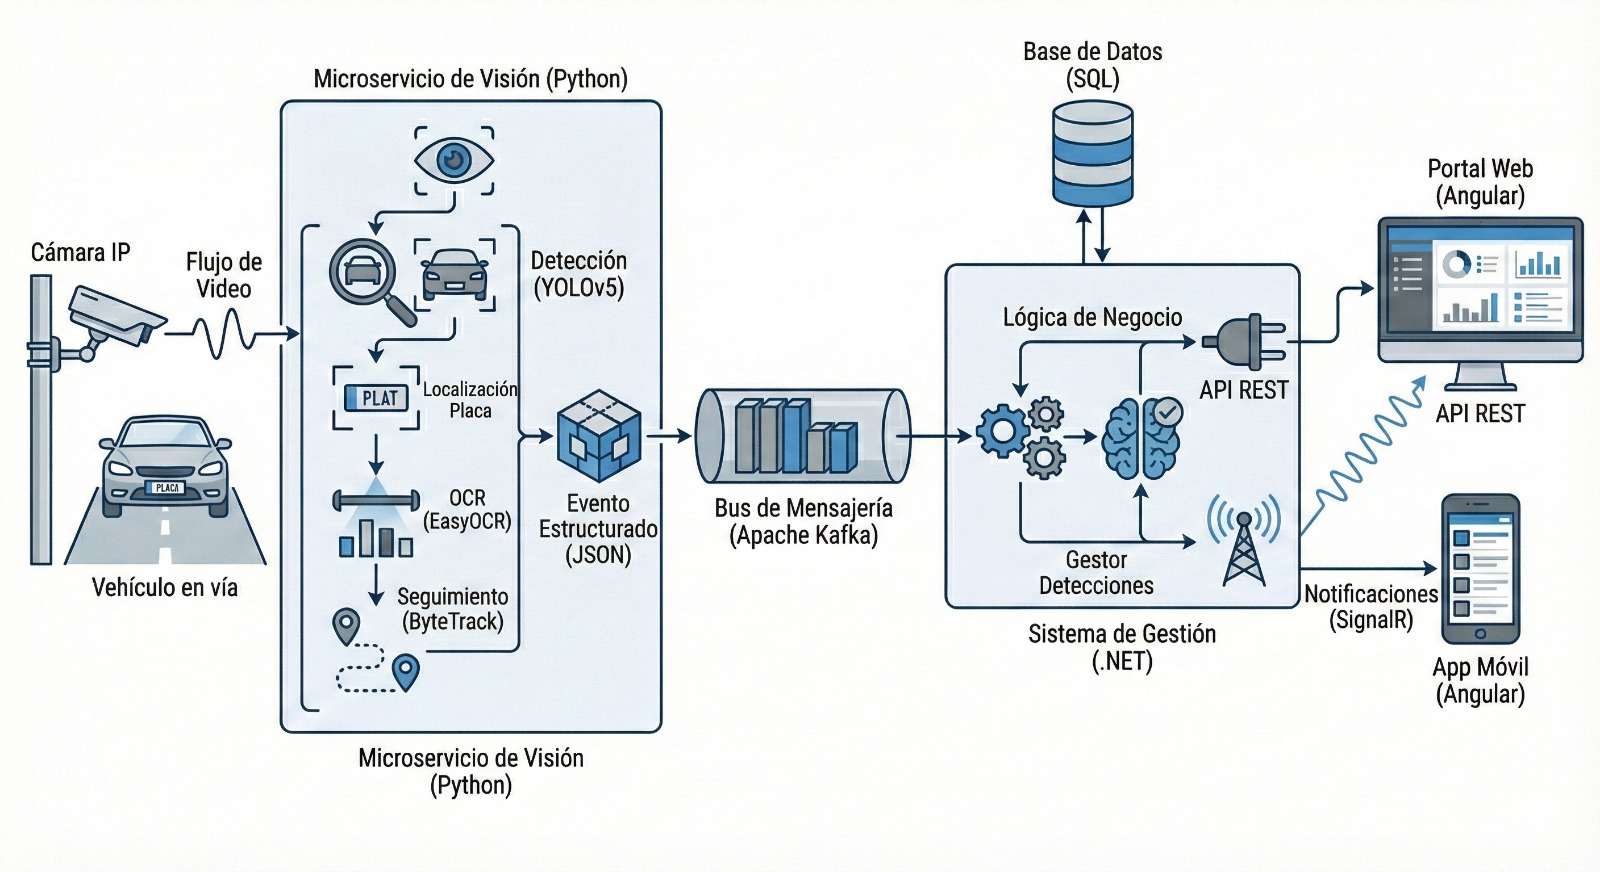
\includegraphics[width=\linewidth]{graphics/implementacion.jpeg}
    \caption{Arquitectura detallada de ANPR-VISION: flujo de información desde la cámara IP hasta el backend de gestión y las interfaces de usuario.}
    \label{fig:arquitectura_detallada_anpr_vision}
\end{figure}
